\paragraph{Search}
\begin{center}
  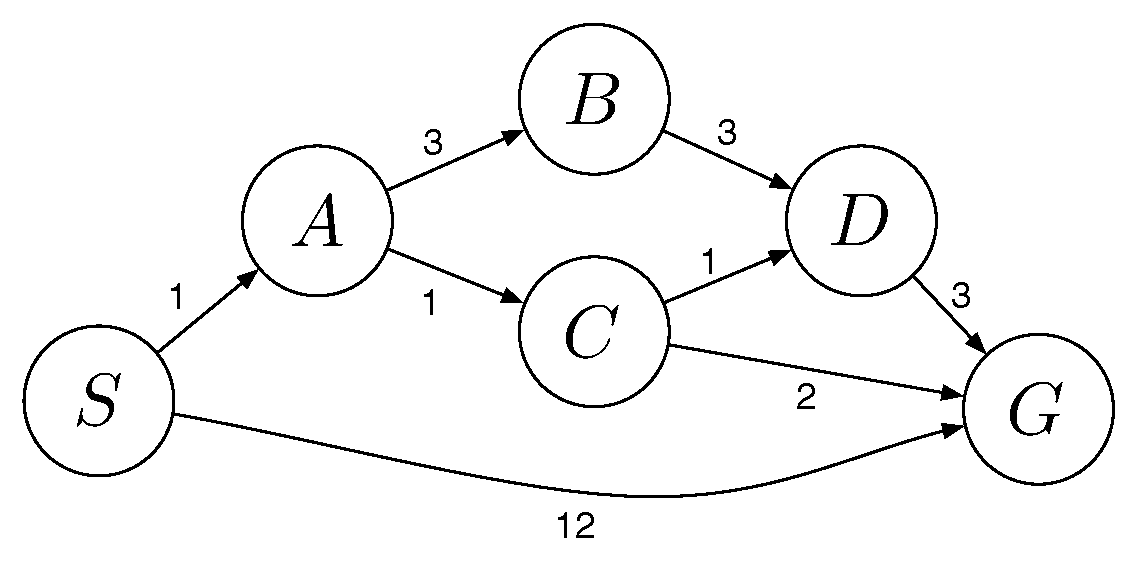
\includegraphics[width=0.6\linewidth]{figures/search_problem.pdf}
\end{center}
Answer the following questions about the search problem shown above. Break any ties alphabetically. For the questions that ask for a path, please give your answers in the form `$S-A-D-G$.'
\begin{enumerate}
  \item What path would breadth-first graph search return for this search problem? (\textbf{15 points})

  {\color{red} $S-G$}

\vspace{1cm}

  \item What path would uniform cost graph search return for this search problem? (\textbf{15 points})

  {\color{red} $S-A-C-G$}

\vspace{1cm}

  \item What path would depth-first graph search return for this search problem? (\textbf{15 points})

  {\color{red} $S-A-B-D-G$}

\vspace{1cm}

  \item What path would A* graph search, using a consistent heuristic, return for this search problem? (\textbf{15 points})

  {\color{red} $S-A-C-G$}

  \newpage

  \item Consider the heuristics for this problem shown in the table below.
  \begin{center}
  \begin{tabular}{|c|c|c|}
    \hline
    State & $h_1$ & $h_2$\\
    \hline
    $S$ & 5 & 4 \\
    \hline
    $A$ & 3 & 2 \\
    \hline
    $B$ & 6 & 6 \\
    \hline
    $C$ & 2 & 1 \\
    \hline
    $D$ & 3 & 3 \\
    \hline
    $G$ & 0 & 0 \\
    \hline
  \end{tabular}
  \end{center}
  \begin{enumerate}
      \item Is $h_1$ admissible? (\textbf{10 points}) \textbf{Yes \hspace{5pt} {\color{red} No}}\\
      Why?
      \vspace{2cm}

      \item Is $h_1$ consistent? (\textbf{10 points}) \textbf{Yes \hspace{5pt} {\color{red} No}}\\
      Why?
      \vspace{2cm}

      \item Is $h_2$ admissible? (\textbf{10 points}) \textbf{{\color{red} Yes} \hspace{5pt} No}\\
      Why?
      \vspace{2cm}

      \item Is $h_2$ consistent? (\textbf{10 points}) \textbf{Yes \hspace{5pt} {\color{red}No}}\\
      Why?
      \vspace{2cm}

  \end{enumerate}

{\color{red}
A heuristic is \textit{admissible} if it never overestimates the cost of reaching the goal, i.e., it is optimistic. Mathematically, for all node $n$, $0\leq h(n)\leq h^*(n)$, where $h^*(n)$ is the optimal cost to reach a goal from node $n$ and $h(n)$ is the cost indicated by the heuristic to reach a goal from node $n$.

\vspace{0.5cm}

A heuristic is \textit{consistent} if its estimate is always less than or equal to the estimated distance from any adjacent node to the goal, plus the cost of reaching that adjacent node. Mathematically, for every node $n1$ and each successor $n2$ of $n1$, $h(n1)-h(n2)\leq c(n1 \rightarrow n2)$, where $c(n1 \rightarrow n2)$ represent the cost of getting to $n2$ from $n1$.

\vspace{0.5cm}

\begin{enumerate}
\item $h1$ overestimates the cost $S \to G$ as $5$ when it is $4$, so it is inadmissible. Note that only one counterexample is enough for finding out that a heuristic is not admissible. 

\item $h1$ is not consistent because $h(S) - h(A) \leq c(S \to A)$ is violated as $5 - 3 \leq 1$. Note that only one counterexample is enough for finding out that a heuristic is not consistent. 

\item $h2$ does not overestimate costs and is admissible. 

\item $h2$ is not consistent because $h(S) - h(A) \leq c(S \to A)$ is violated as $4 - 2 \leq 1$.
\end{enumerate}

}

\end{enumerate}
